
% ============================================================
%  Příprava na maturitu – Elektrotechnika
%  Okruh 10: Elektroinstalace a ochrana před bleskem
% ============================================================

\documentclass[a4paper,10pt]{article}

\usepackage[T1]{fontenc}
\usepackage[utf8]{inputenc}
\usepackage[left=2.0cm, right=1.8cm, top=1.8cm, bottom=1.8cm]{geometry}
\usepackage{parskip}
\usepackage{xcolor}
\usepackage{tabularx}
\usepackage{booktabs}
\usepackage{tikz}
\usepackage{mdframed}
\usepackage{amsmath}
\usepackage{enumitem}
\usepackage{circuitikz}

\usetikzlibrary{arrows.meta, positioning, decorations.pathmorphing, shapes.geometric, calc}

% --- Barvy ---
\definecolor{accent}{HTML}{1A3A5C}
\definecolor{lightblue}{HTML}{EAF2F8}
\definecolor{lightyellow}{HTML}{FDFBE4}
\definecolor{lightgreen}{HTML}{EAF7EA}
\definecolor{lightred}{HTML}{FDE8E8}
\definecolor{lightgray}{HTML}{F4F4F4}

% --- Boxy ---
\newmdenv[backgroundcolor=lightblue,linecolor=accent!40,roundcorner=4pt,
  innertopmargin=6pt,innerbottommargin=6pt,innerleftmargin=8pt,innerrightmargin=8pt]{pojmybox}
\newmdenv[backgroundcolor=lightyellow,linecolor=accent!30,roundcorner=4pt,
  innertopmargin=6pt,innerbottommargin=6pt,innerleftmargin=8pt,innerrightmargin=8pt]{vysvetlenibox}
\newmdenv[backgroundcolor=lightgreen,linecolor=accent!40,roundcorner=4pt,
  innertopmargin=6pt,innerbottommargin=6pt,innerleftmargin=8pt,innerrightmargin=8pt]{vzorcebox}
\newmdenv[backgroundcolor=lightred,linecolor=accent!30,roundcorner=4pt,
  innertopmargin=6pt,innerbottommargin=6pt,innerleftmargin=8pt,innerrightmargin=8pt]{durazbox}

\setlist[itemize]{noitemsep, leftmargin=1.4em, topsep=2pt}
\setlist[enumerate]{noitemsep, leftmargin=1.4em, topsep=2pt}

% --- Zkratka pro jednotky ---
\newcommand{\jednotka}[1]{\,[\mathrm{#1}]}

\begin{document}

% ============================================================
\section*{\large Okruh 10 – Elektroinstalace a ochrana před bleskem}

\begin{pojmybox}
\textbf{Klíčové pojmy:}
elektroinstalace, vodiče a kabely, sítě TN-C / TN-S, ochranný vodič (PE), střední vodič (N), fázový vodič (L), uzemnění, pospojování, hromosvod (LPS), svodiče přepětí (SPD), krokové napětí
\end{pojmybox}

\begin{vysvetlenibox}

% ================================================================
\subsection*{1. Vodiče a kabely v elektroinstalaci}

Základem domovních i průmyslových rozvodů jsou měděné (dříve hliníkové) vodiče. Každý vodič má svou jasně definovanou barvu, která se \textbf{nesmí zaměnit}:

\begin{itemize}
    \item \textbf{Fázový vodič (L - Line):} Hnědá, černá, šedá. Vodič, na kterém je nebezpečné napětí (230 V proti zemi).
    \item \textbf{Střední / Nulový vodič (N - Neutral):} Světle modrá. Pracovní vodič, který uzavírá obvod. Teoreticky je na něm potenciál země (0 V), ale protéká jím pracovní proud.
    \item \textbf{Ochranný vodič (PE - Protective Earth):} \textbf{Zeleno-žlutá.} Slouží výhradně k ochraně před úrazem (připojuje se na neživé kovové kryty spotřebičů). Za normálního stavu jím neprotéká žádný proud!
\end{itemize}

\textbf{Značení kabelů (příklady):}
\begin{itemize}
    \item \textbf{CYKY:} Pevný instalační kabel pod omítku (např. CYKY-J 3x1,5 pro světla, CYKY-J 3x2,5 pro zásuvky).
    \item \textbf{CYSY:} Ohebný kabel pro pohyblivé přívody (prodlužovačky, připojení spotřebičů).
\end{itemize}

% ================================================================
\subsection*{2. Druhy sítí nízkého napětí}

V Evropě se nejčastěji používají sítě typu \textbf{TN} (Terra-Neutral). Písmena určují vztah sítě k zemi a provedení ochranného vodiče.

\begin{enumerate}
    \item \textbf{TN-C (Combined):} Ochranný (PE) a střední (N) vodič jsou sloučeny do jednoho společného vodiče \textbf{PEN} (zeleno-žlutý). Třívodičová soustava (L1, L2, L3, PEN). \textit{Staré instalace. Nebezpečné při přerušení vodiče PEN!}
    \item \textbf{TN-S (Separated):} Ochranný (PE) a střední (N) vodič jsou od transformátoru vedeny \textbf{odděleně}. Pětivodičová soustava (L1, L2, L3, N, PE). \textit{Moderní a bezpečná instalace, nutná pro funkci proudových chráničů.}
    \item \textbf{TN-C-S:} Nejběžnější praxe. K budově přijde síť TN-C (čtyři dráty) a v hlavním rozváděči se vodič PEN \textbf{rozdělí} na PE a N. Od tohoto bodu dále už je síť TN-S.
\end{enumerate}

\begin{center}
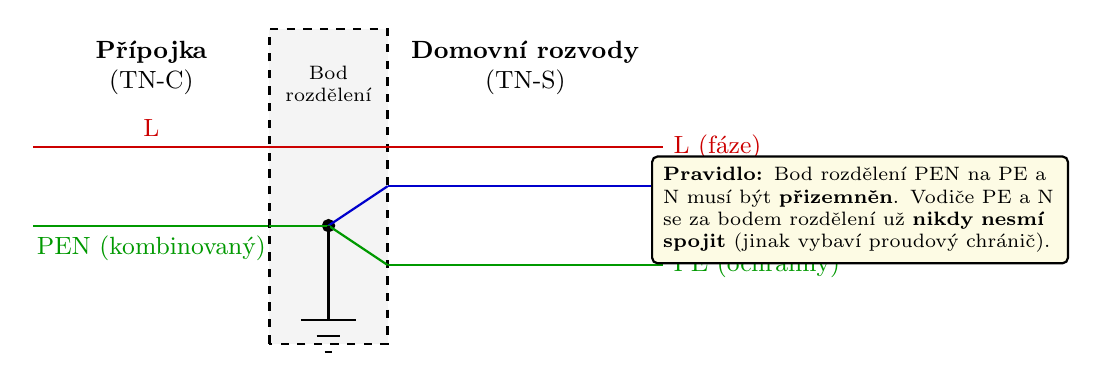
\begin{tikzpicture}[>=Stealth, font=\small, thick]
  % Síť TN-C
  \draw[red!80!black] (0,2) -- (3,2) node[midway, above] {L};
  \draw[green!60!black] (0,1) -- (3,1) node[midway, below] {PEN (kombinovaný)};
  
  \node[align=center] at (1.5, 3) {\textbf{Přípojka}\\(TN-C)};

  % Bod rozdělení
  \draw[fill=lightgray, dashed] (3,-0.5) rectangle (4.5,3.5);
  \node[align=center, font=\scriptsize] at (3.75, 2.8) {Bod\\rozdělení};
  
  \filldraw[black] (3.75, 1) circle (2pt);
  \draw[green!60!black] (3,1) -- (3.75,1);
  \draw[blue!80!black] (3.75,1) -- (4.5,1.5);
  \draw[green!60!black] (3.75,1) -- (4.5,0.5);
  
  % Přizemnění bodu rozdělení
  \draw (3.75, 1) -- (3.75, -0.2);
  \draw (3.4, -0.2) -- (4.1, -0.2);
  \draw (3.6, -0.4) -- (3.9, -0.4);
  \draw (3.7, -0.6) -- (3.8, -0.6);

  % Síť TN-S
  \draw[red!80!black] (3,2) -- (4.5,2) -- (8,2) node[right] {L (fáze)};
  \draw[blue!80!black] (4.5,1.5) -- (8,1.5) node[right] {N (pracovní)};
  \draw[green!60!black] (4.5,0.5) -- (8,0.5) node[right] {PE (ochranný)};
  
  \node[align=center] at (6.25, 3) {\textbf{Domovní rozvody}\\(TN-S)};
  
  \begin{scope}[xshift=8.5cm, yshift=0.5cm]
    \node[align=left, text width=5cm, font=\scriptsize, draw, fill=lightyellow, rounded corners=2pt, inner sep=4pt] at (2,0.7) {
      \textbf{Pravidlo:} Bod rozdělení PEN na PE a N musí být \textbf{přizemněn}. Vodiče PE a N se za bodem rozdělení už \textbf{nikdy nesmí spojit} (jinak vybaví proudový chránič).
    };
  \end{scope}
\end{tikzpicture}
\end{center}

% ================================================================
\subsection*{3. Uzemnění a pospojování}

Uzemnění znamená vodivé spojení částí elektrického zařízení se zemí pomocí \textbf{zemniče}.

\begin{itemize}
    \item \textbf{Zemniče:} Vkládají se do země. Dělí se na náhodné (např. ocelové armatury v betonu) a strojené (páskové, tyčové, základový zemnič).
    \item \textbf{Hlavní pospojování (MET/EPS):} Všechny kovové části v budově (trubky vody, topení, plynu, vany, konstrukce) se musí vodivě pospojovat a připojit na hlavní zemnicí svorkovnici. Zabraňuje to vzniku nebezpečného rozdílu potenciálů (napětí) mezi těmito předměty.
\end{itemize}

% ================================================================
\subsection*{4. Ochrana před bleskem – Vnější (LPS)}

Blesk je obrovský elektrický výboj (až 100 kA, miliony voltů). Vnější systém ochrany (LPS - Lightning Protection System), laicky \textbf{hromosvod}, slouží k zachycení blesku a jeho svedení do země tak, aby nezpůsobil požár nebo mechanické poškození budovy.

\textbf{Skládá se ze 3 částí:}
\begin{enumerate}
    \item \textbf{Jímač:} Zachytává úder blesku (tyčové, hřebenové mříže na střeše).
    \item \textbf{Svod:} Nejkratší a nejpřímější cestou svádí bleskový proud od jímače k zemniči (vede se po fasádě nebo pod ní).
    \item \textbf{Zemnič:} Bezpečně rozptýlí energii do země.
\end{enumerate}

\begin{center}
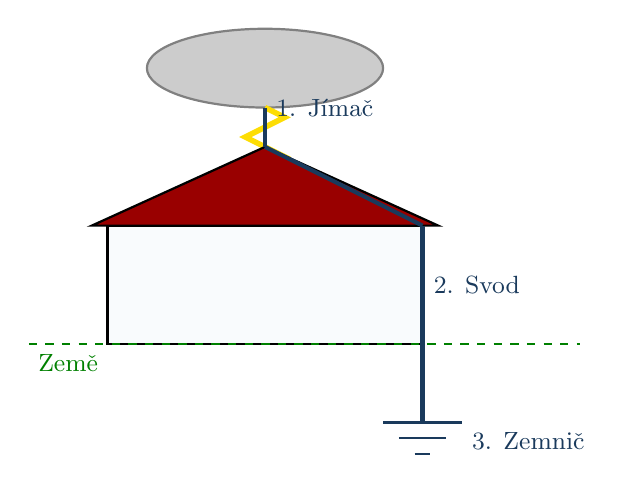
\begin{tikzpicture}[>=Stealth, font=\small, thick]
  % Mrak a blesk
  \draw[fill=gray!40, draw=gray] (1,3.5) ellipse (1.5 and 0.5);
  \draw[yellow!80!orange, line width=2pt, decorate, decoration={zigzag, segment length=5mm, amplitude=2.5mm}, ->] (1,3) -- (1,1.8);
  
  % Budova
  \draw[fill=lightblue!30] (-1,0) rectangle (3,1.5);
  \draw[fill=red!60!black] (-1.2,1.5) -- (1,2.5) -- (3.2,1.5) -- cycle;
  
  % Hromosvod
  \draw[line width=1.5pt, accent] (1,2.5) -- (1,3) node[right] {1. Jímač}; % Jímač
  \draw[line width=1.5pt, accent] (1,2.5) -- (3,1.5); % Po střeše
  \draw[line width=1.5pt, accent] (3,1.5) -- (3,0) node[midway, right] {2. Svod}; % Svod
  
  % Zemnič
  \draw[line width=1.5pt, accent] (3,0) -- (3,-1);
  \draw[accent] (2.5,-1) -- (3.5,-1) node[below right] {3. Zemnič};
  \draw[accent] (2.7,-1.2) -- (3.3,-1.2);
  \draw[accent] (2.9,-1.4) -- (3.1,-1.4);
  
  % Zem
  \draw[green!50!black, dashed] (-2,0) -- (5,0);
  \node[green!50!black, below] at (-1.5,0) {Země};
\end{tikzpicture}
\end{center}

\begin{durazbox}
\textbf{Krokové napětí:} Pokud blesk uhodí do země (nebo do zemniče), proud se radiálně šíří zemí. Půda má elektrický odpor, takže mezi různými body na zemi vzniká úbytek napětí. Rozkročí-li se člověk (či zvíře) blízko místa úderu, vznikne mezi jeho nohama nebezpečné \textbf{krokové napětí} a proud projde tělem.
\end{durazbox}

% ================================================================
\subsection*{5. Ochrana před přepětím – Vnitřní (SPD)}

Blesk nemusí uhodit přímo do domu. I úder stovky metrů daleko vyvolá obrovské \textbf{elektromagnetické pole}, které v elektrických rozvodech indukuje přepěťové špičky (tisíce voltů). Ty okamžitě zničí citlivou elektroniku (TV, PC, routery).

K ochraně se používají \textbf{Svodiče přepětí (SPD - Surge Protection Device)}. Tyto přístroje fungují jako "ventil". Za normálního napětí (230 V) jsou nevodivé. Jakmile napětí překročí nebezpečnou mez, svodič se okamžitě otevře a přepěťovou vlnu odvede do uzemnění (PE).

\textbf{Třístupňová ochrana (Koordinace SPD):}
\begin{itemize}
    \item \textbf{Typ 1 (Bleskojistka / T1):} Zachycuje nejhrubší energii (přímý úder blesku). Instaluje se v \textbf{hlavním rozváděči}.
    \item \textbf{Typ 2 (Varistor / T2):} Instaluje se v \textbf{podružném (bytovém) rozváděči}. Ořezává napětí na cca 1,5 kV.
    \item \textbf{Typ 3 (Jemná ochrana / T3):} Instaluje se přímo k zařízení (v zásuvkách, v prodlužovačkách). Chrání konkrétní citlivý spotřebič.
\end{itemize}

% ================================================================
\subsection*{6. Shrnutí – Barvy vodičů v instalaci}

\begin{center}
\begin{tabularx}{0.97\linewidth}{@{} l l X @{}}
\toprule
\textbf{Značka} & \textbf{Funkce} & \textbf{Předepsaná barva} \\
\midrule
\textbf{L (L1, L2, L3)} & Fázový vodič (pracovní) & Hnědá, Černá, Šedá \\
\textbf{N} & Střední vodič (pracovní) & Světle modrá \\
\textbf{PE} & Ochranný vodič & Zeleno-žlutá pruhovaná \\
\textbf{PEN} & Kombinovaný vodič (ochr. i prac.) & Zeleno-žlutá pruhovaná \\
\bottomrule
\end{tabularx}
\end{center}

\end{vysvetlenibox}

\end{document}
